\subsection{Task 1.1.3: Local Linear Models}

In diesem Beispiel ist die Designmatrix X doppelt so groß wie vorher. War sie in Task 1.1.2 noch $(60 \times d)$ groß, ist sie jetzt $(60 \times 2d)$. Neben den unskalierten Gausskurven gibt es nun auch ein zweites Set von Basisfunktionen: die Gausskurven von vorher, linear skaliert mit $x$.

Die Implementierung in Matlab ist der von Task 1.1.2 sehr ähnlich, es wurde nur eine zweite Designmatrix generiert, die der normalen Designmatrix entspricht, aber mit $x$ multipliziert wurde. Mit dem Klammer-Operator \texttt{[]} wurden die beiden Matrizen dann zu einer Matrix verbunden.

Abbildung~\ref{fig:113-curves-out} zeigt die Datenpunkte, die tatsächliche Funktion und die gelernte Funktion für unterschiedliche Anzahl von Basisfunktionen. Man erkennt, dass die Annäherung bei einer geringen Anzahl von Basisfunktionen nicht besonders gut ist, aber dann mit steigender Anzahl von Basisfunktionen sehr gut wird. Ist jedoch die Anzahl zu hoch, wird die Annäherung auch sehr schlecht.

Da Abbildung~\ref{fig:113-curves-out} auf alle Kurven skaliert wurde, erkennt man die angenäherte Funktion nicht besonders gut. Abbildung~\ref{fig:113-curves-in} zeigt die gleichen Kurven bei einer sinnvolleren Skalierung.

\begin{figure}[h!]
  \centering
  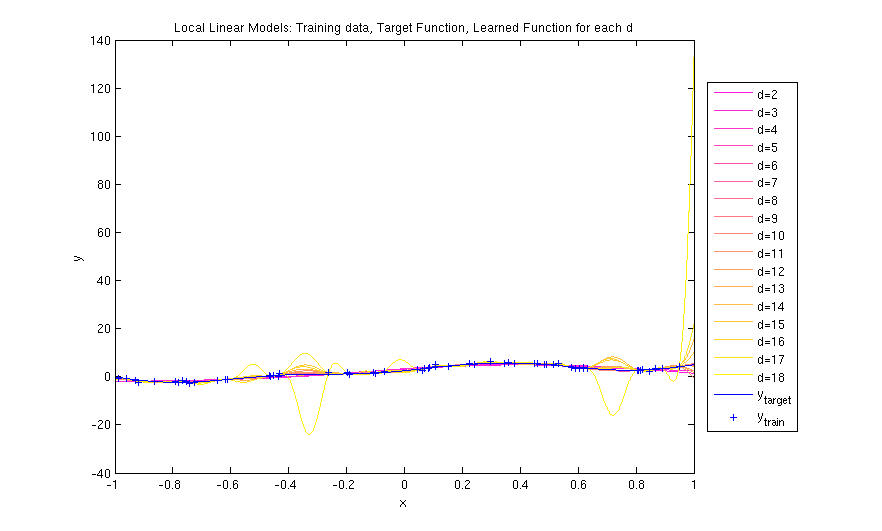
\includegraphics[width=\textwidth]{./figures/1_1_3_curves_out.png}
  \caption{Trainings-Punkte, Target-Funktion \& gelernte Funktion}
  \label{fig:113-curves-out}
\end{figure}

\begin{figure}[h!]
  \centering
  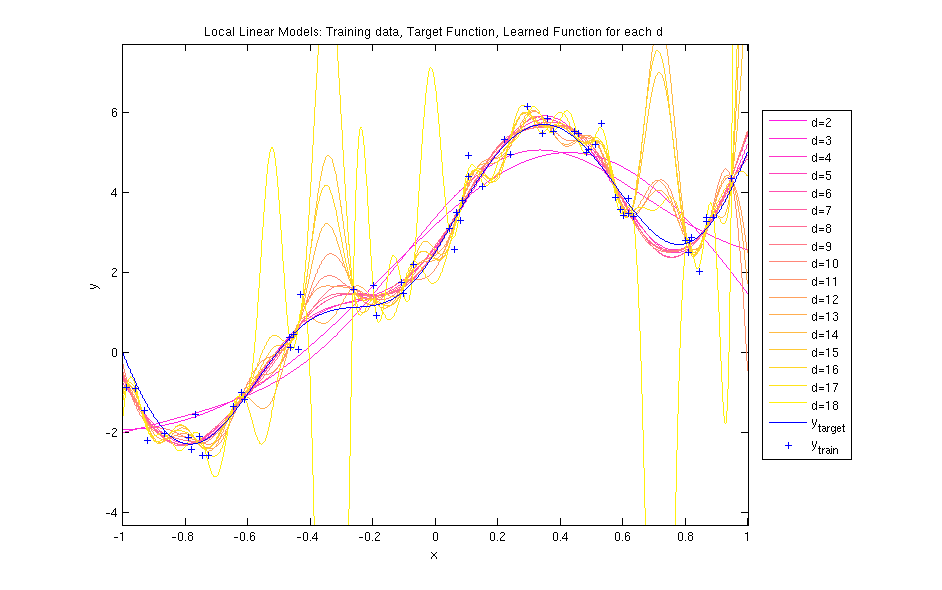
\includegraphics[width=\textwidth]{./figures/1_1_3_curves_in.png}
  \caption{Trainings-Punkte, Target-Funktion \& gelernte Funktion (skaliert)}
  \label{fig:113-curves-in}
\end{figure}

Diese Kurven sind aus einer gewissen Anzahl Basisfunktionen zusammengestellt, wobei die folgenden Abbildung diese Basisfunktionen visualisieren. Abbildung~\ref{fig:113-basis-6} zeigt die Verteilung von 6 Basisfunktionen, Abbildung~\ref{fig:113-basis-12} zeigt die Verteilung von 12 Basisfunktionen und Abbildung~\ref{fig:113-basis-18} zeigt die Verteilung von 18 Basisfunktionen.

\begin{figure}[h!]
  \centering
  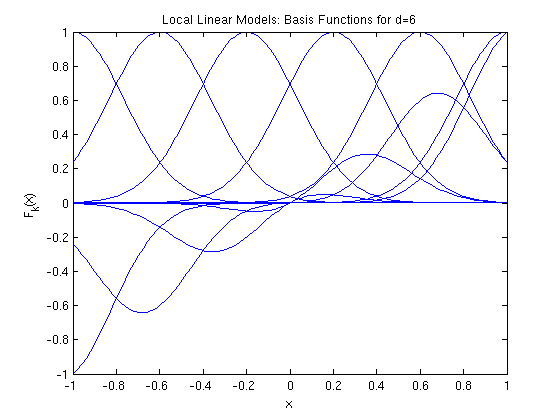
\includegraphics[width=0.75\textwidth]{./figures/1_1_3_basis_6.png}
  \caption{Aufteilung von 6 Basisfunktionen $\Phi_k(x)$}
  \label{fig:113-basis-6}
\end{figure}

\begin{figure}[h!]
  \centering
  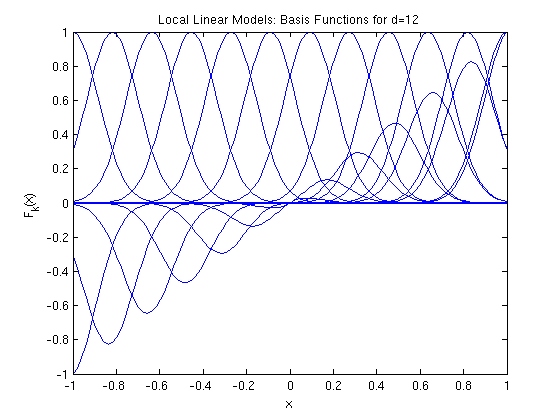
\includegraphics[width=0.75\textwidth]{./figures/1_1_3_basis_12.png}
  \caption{Aufteilung von 12 Basisfunktionen $\Phi_k(x)$}
  \label{fig:113-basis-12}
\end{figure}

\begin{figure}[h!]
  \centering
  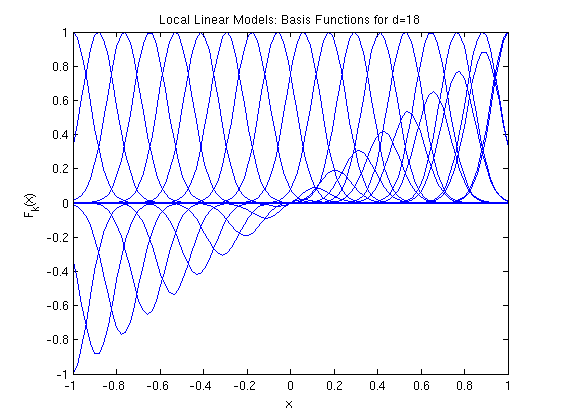
\includegraphics[width=0.75\textwidth]{./figures/1_1_3_basis_18.png}
  \caption{Aufteilung von 18 Basisfunktionen $\Phi_k(x)$}
  \label{fig:113-basis-18}
\end{figure}

Abbildung~\ref{fig:113-mse-out} zeigt den Mean Squared Error (MSE) bei den Trainings- und Testdaten in Abhängigkeit von der Anzahl der Basisfunktionen. Wie man auch in Abbildung~\ref{fig:113-curves-out} und Abbildung~\ref{fig:113-curves-in} erkennt, funktioniert die Annäherung für mittelgroße Werte von $l$ (Anzahl der Basisfunktionen) am besten. In Abbildung~\ref{fig:113-mse-out} erkennt man, wie extrem schlecht die Annäherung mit großen $l$ funktioniert. Passend skaliert ist der MSE in Abbildung~\ref{fig:113-mse-in} dargestellt. Ein sehr niedriger MSE ist bei $l=4$ Basisfunktionen erreichbar, wodurch durch den niedrigen Grad auch nur ein geringer Aufwand entsteht.

\begin{figure}[h!]
  \centering
  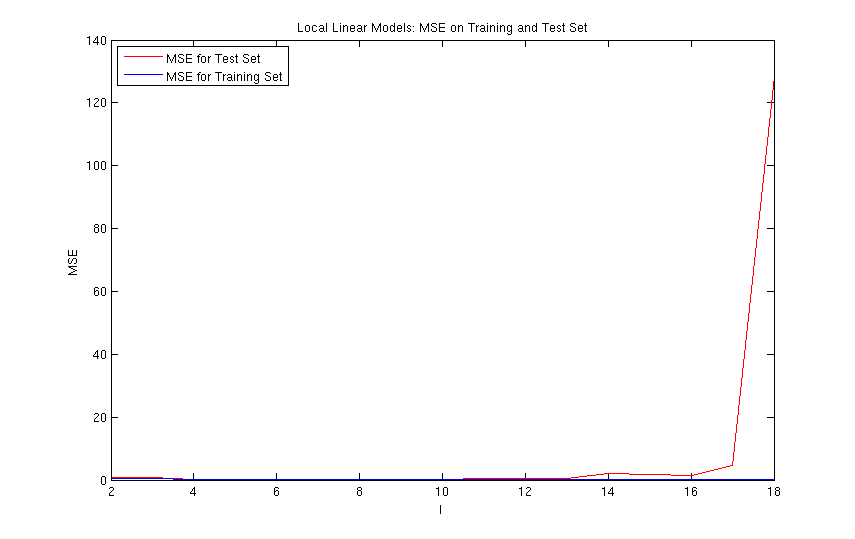
\includegraphics[width=\textwidth]{./figures/1_1_3_mse_out.png}
  \caption{MSE in Abhängigkeit von $l$}
  \label{fig:113-mse-out}
\end{figure}

\begin{figure}[h!]
  \centering
  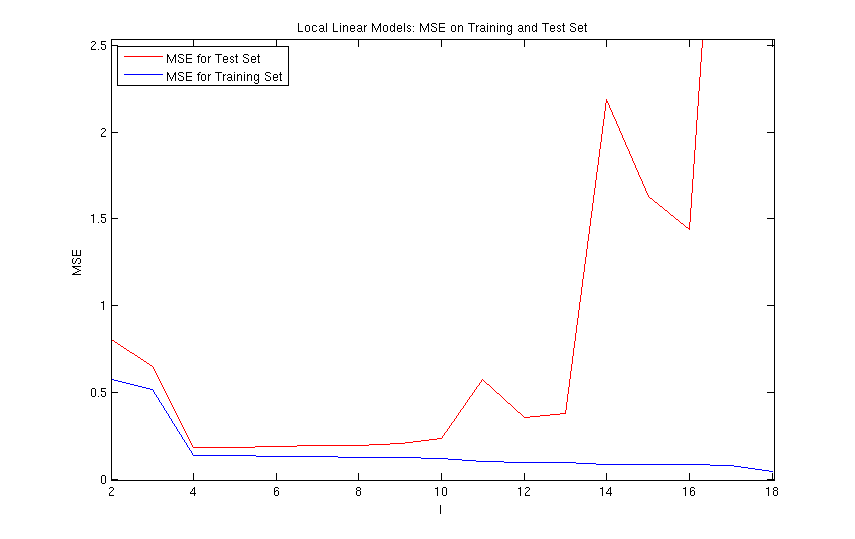
\includegraphics[width=\textwidth]{./figures/1_1_3_mse_in.png}
  \caption{MSE in Abhängigkeit von $l$ (skaliert)}
  \label{fig:113-mse-in}
\end{figure}

\clearpage

\paragraph{Vergleich zwischen den verschiedenen Basisfunktionen}

Den kleinsten MSE lieferten die Basisfunktionen in Task 1.1.2 und 1.1.3, wobei bei Task 1.1.2 die Gesamtperformance
über alle Ordnungen betrachtet sehr gut war. Bei Task 1.1.1 wird ein ähnlich gutes Ergebnis erst ab höherer Ordnung
erzielt. Die Basisfunktionen aus Task 1.1.3 ist für niedrigen Ordnungen bis ca. 12 gut, aber wird danach ziehmlich
schnell unbrauchbar. Für höhere Ordnung empfiehlt es sich den in Task 1.1.4 beschriebenen Faktor $\alpha$ einzuführen.
